\subsection{Objektmodel}

For at få overblik over virksomheden og hvorledes deres timesedler virker begyndte vi med en objektmodel.
Vores objektmodel er blevet opbygget ud fra møder med Firmaet, og er blevet ændret undervejs, deribland efter en diskussion med en vejleder.

Den første objektmodel var opbygget ud fra use casen "Registrering af timer".
Over projektet har modellen gennemgået flere iterationer, og flere objekter er blevet tilføjet i trin med at vi har opdaget dem, eller evt. skulle arbejde med dem.
Ligeledes er der også blevet fjernet objekter, som var relevante til firmaet, men ikke havde relevans til programmet og kun gjorde modellen for kompleks

De første iterationer havde flere objekter såsom et Bygma objekt, hvor Bygma er en leverandør af træ til Halvorsen ApS. Bygma har dog ikke haft behov for at blive repræsenteret i modellen, da vi aldrig bruger dem til timeregistrering.
Ligeledes havde vi også et værkstedsobjekt, som var irrelevant i forhold til at kunne registrere sine timer digitalt.

I de første iterationer havde mange objekter forbindelser til flere forskellige objekter, som skabte et uoverskueligt spindelvæv af forbindelser, da alle vores objekter havde en eller slags reference til hinanden. 

Vi spurgte vores systemudviklings underviser Tove til råds om, hvad vi skulle gøre. Hun forklarede at objektmodellen ikke nødvendigvis behøvede at vise alle referencerne mellem objekterne, men kun dem, som var nødvendige for systemet.

I modellen ses der alle objekterne vi havde behov for at modellere i forhold til programmet. Vores objektmodel kan ses på figur \ref{fig:Objektmodel}.

\begin{figure}[H]
    \makebox[\textwidth][c]{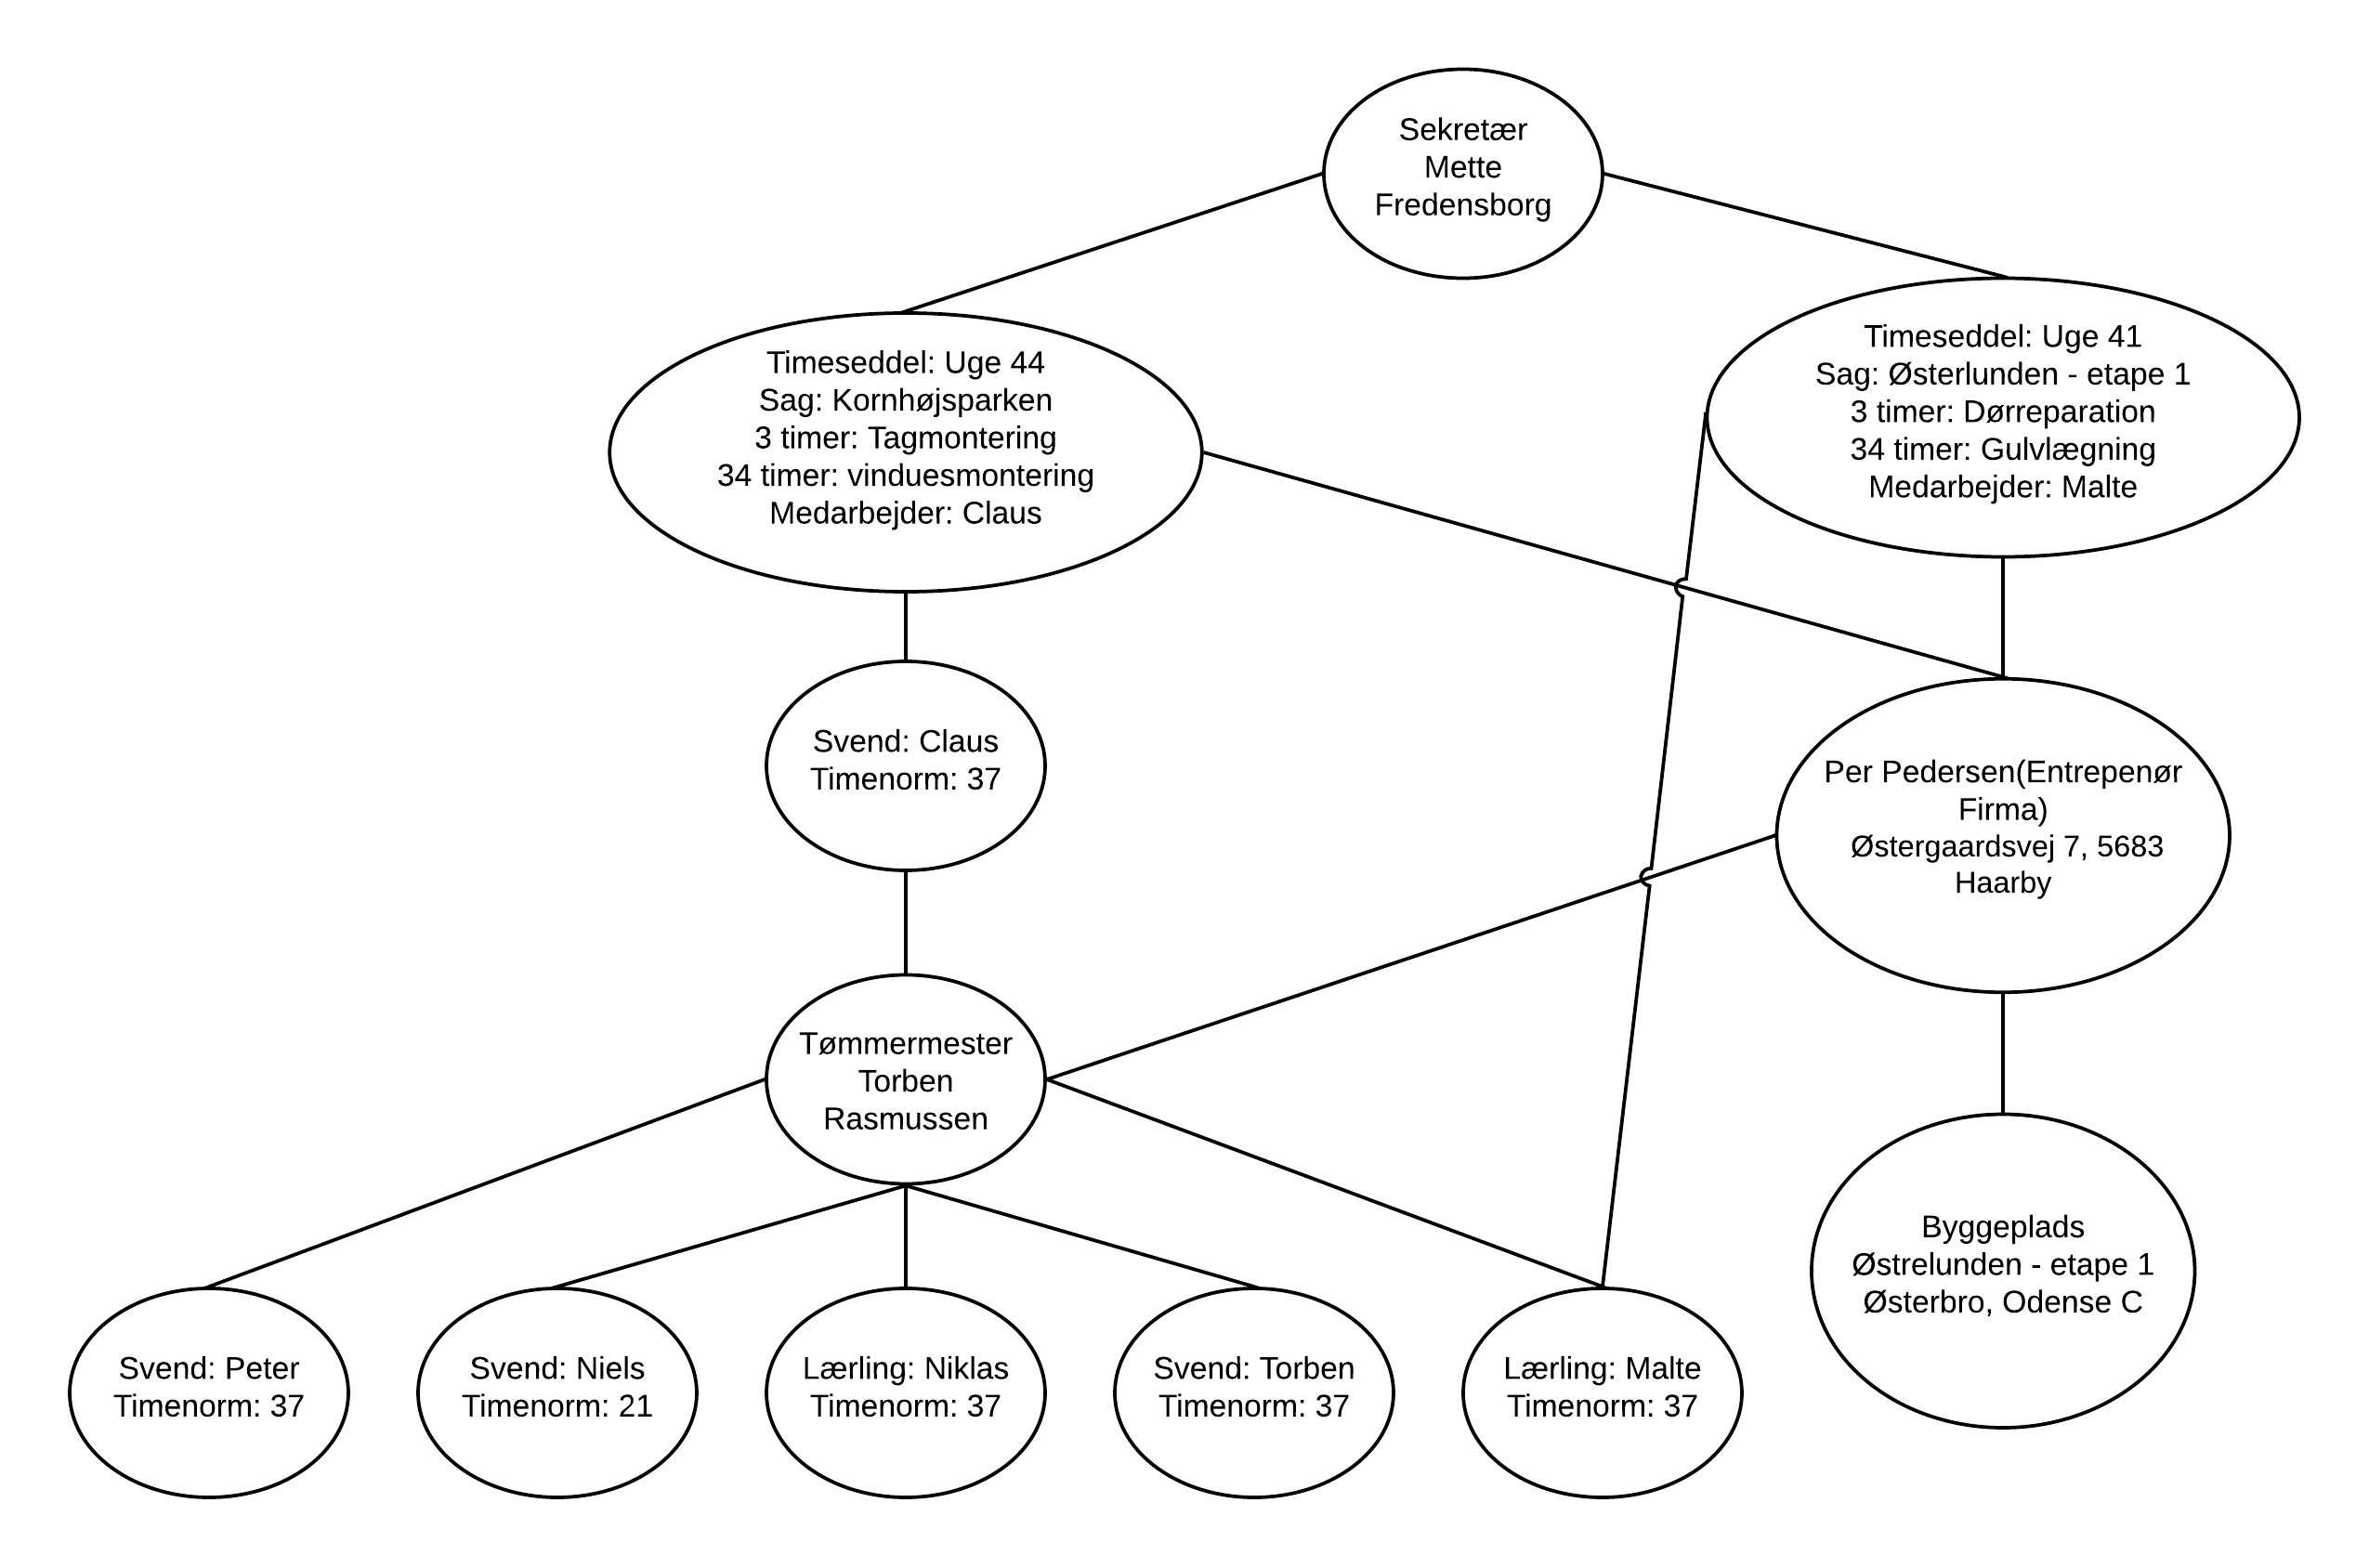
\includegraphics[scale = .6]{ObjektModelSprint2.png}}
    \caption{Objektmodel}
    \label{fig:Objektmodel}
\end{figure}

Der findes flere forskellige objekter. Størstedelen af objekterne er medarbejder objekter. De resterende er timeseddel objekter, byggeplads objekter og kunde objekter. 